\begin{figure}
\begin{tabular}{cc}
\begin{subfigure}[b]{0.45\textwidth}
\begin{center}
{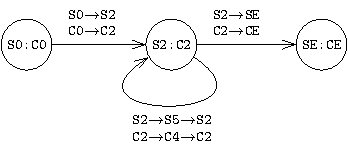
\includegraphics[scale=1.1]{chapters/figures/figSumListProductCfg.pdf}}
\end{center}
\caption{\label{fig:llTraverseProduct}Product-CFG}
\end{subfigure}%
&
\begin{subfigure}[b]{0.55\textwidth}
\begin{center}
\begin{footnotesize}
\begin{tabular}{|c|l|}
\hline
{\bf PC-Pair} & \multicolumn{1}{c|} {\bf Invariants} \\
\hline
\hline
(\scpc{0}{0}) &
\Tstrut $\circled{P}\  \sv{l} \indEq{} \lifted{list}{\mem{}}{lnode}{\cv{l}}$ \\
\multirow{2}{*}{(\scpc{2}{2})} &
\Tstrut $\circled{\scriptsize I1}\  \sv{l} \indEq{} \lifted{list}{\mem{}}{lnode}{\cv{l}}$ \\ &
\Tstrut $\circled{\scriptsize I2}\  \sv{sum} = \cv{sum}$ \\
(\scpc{E}{E}) &
\Tstrut $\circled{\scriptsize E}\  \sv{ret} = \cv{ret}$ \\
\hline
\end{tabular}
\end{footnotesize}
\vspace{13px}
\end{center}
\caption{\label{fig:llTraverseProductInv}Node Invariants of the Product-CFG}
\end{subfigure}%
\\
\end{tabular}
\caption{\label{fig:llTraverseProductCFGInvs} Product-CFG between the IRs in \cref{fig:llTraverseSpecIR,fig:llTraverseCIR}. The inductive invariants of the Product-CFG are given in \cref{fig:llTraverseProductInv}.}
\end{figure}
